	\subsection{Définitions et généralités}
		
Un graphe non orienté G est la donnée d’un couple (V , E) où V = \{$ \textit{v}_{1} , \textit{v}_{2} ,..., \textit{v}_{n} $\} est un ensemble fini dont les éléments sont appelés sommets ou nœuds ( Vertices en anglais ) et  E=\{$\textit{e}_{1} ,  \textit{e}_{2} ,…, \textit{e}_{m} $\} est un ensemble fini d'arêtes ( Edges en anglais ). Toute arête \textit{e} de E correspond à un couple non ordonné de sommets ( $\textit{v}_{i} , \textit{v}_{j}$ ) $\in$ E $\subset$  $V \times V$ représentant ses extrémités \citep{muller} \citep{fages2014exploitation}.
\\Soient \textit{e} = ($\textit{v}_{i} , \textit{v}_{j}$) et \textit{e'}=($\textit{v}_{k} , \textit{v}_{l}$) deux arêtes de E, On dit que :
\begin{itemize}
\item $\textit{v}_{i}$ et $\textit{v}_{j}$ sont les extrémités de \textit{e} et \textit{e} est incidente à $\textit{v}_{i}$ et $\textit{v}_{j}$ \citep{hennecart2012elements}.
\item $\textit{v}_{i}$ et $\textit{v}_{j}$ sont voisins ou adjacents, s'il y a au moins une arête entre eux dans E \citep{IUTLyonInformatique}.
\item L'ensemble des sommets adjacents aux deux extrémités de \textit{e} est appelé le voisinage de \textit{e} \citep{muller}. 
\item \textit{e} et \textit{e'} sont voisins s'ils ont une extrémité commune  \citep{lopez2003cours}.
\item L'arête \textit{e} est une boucle si ses extrémités coïncident, i.e, $\textit{v}_{i}$ = $\textit{v}_{j}$ \citep{IUTLyonInformatique}. 
\item L'arête \textit{e} est multiple si elle a plus d'une seule occurrence dans l'ensemble E.
\end{itemize}	
		 
\subsection{Représentation graphique}
Un graphe non orienté G peut être représenté par un dessin sur un plan comme suit \citep{muller}:

\begin{itemize}
\item Les nœuds $\textit{v}_{i}$ $\in$ V de G sont représentés par des points distincts.
\item 	Les arêtes \textit{e} = ($\textit{v}_{i}$,$\textit{v}_{j}$) $\in$ E de G sont représentés par des lignes, pas forcement rectilignes, qui relient les extrémités de chaque arête \textit{e}.
\end{itemize}

%% L'exemple de la représentation graphique 
\textbf{Exemple :}
 Soit g=(V1 , E1) un graphe non orienté tel que : V1=\{ 1,2,3,4,5 \} et E1=\{(1,2), (1,4), (2,2), (2,3), (2,5), (3,4)\}.
La représentation graphique de g est alors donnée par le schéma de la figure \ref{graphNonOriente}.
\\
\begin{figure}[H]
\begin{center}
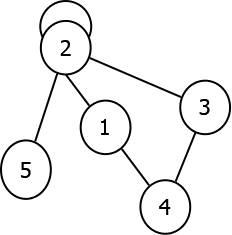
\includegraphics[height=120 pt, width=130 pt]{./ressources/image/graphNonOriente.png} 
\end{center}
\caption{Exemple de représentation graphique d'un graphe non orienté}
\label{graphNonOriente}
\end{figure}

		\subsection{Propriétés d'un graphe}
		
		\begin{itemize}[label=$\circ$]
			
			\item \textbf{Ordre d'un graphe:} On appelle ordre d’un 					graphe le nombre de ses sommets, i.e, Card(V) \citep{DUT}.
			
			\item  \textbf{Taille d'un graphe:} On appelle taille d’un 				graphe le nombre de ses arêtes, i.e, Card(E) \citep{DUT}.
			
			\item  \textbf{Degré dans un graphe:}
			
			
			\begin{itemize}[label=$\bullet$]
				\item \textbf{Degré d'un sommet : } Le degré d’un sommet noté \textit{d}($\textit{v}_{i}$) est le nombre d'arêtes incidentes à ce sommet, sachant qu’une boucle compte pour deux \citep{muller}. Dans l'exemple de la figure \ref{graphNonOriente}, le degré du sommet (1) est : \textit{d}(1)=2.
				
				\item \textbf{Degré d'un graphe : }Le degré d’un graphe est le degré maximum de ses sommets, i.e, max(\textit{d}($\textit{v}_{i}$)) \citep{muller}. Dans l’exemple de 				la figure \ref{graphNonOriente}, le degré du graphe g est \textit{d}(2)=5.
			\end{itemize}
			
			\item \textbf{Rayon et diamètre dans un graphe:}
			\begin{itemize}[label=$\bullet$]
				\item \textbf{Distance : }La distance entre deux sommets 	\textit{v} et \textit{u} est le plus petit nombre d’arêtes qu’on doit parcourir pour aller de \textit{v} à \textit{u} ou de \textit{u} à \textit{v} \citep{muller}. 
				
				\item 	\textbf{Diamètre d’un graphe :} C’est la plus grande 	distance entre deux sommets de ce graphe \citep{muller}. 
				
				\item 	\textbf{Rayon d’un graphe : }C’est la plus petite distance entre deux sommets de ce graphe \citep{parlebas1972centralite}. 
			\end{itemize}
		\end{itemize}
		
	
			
	